\documentclass{beamer}
\usetheme{metropolis}
\usepackage{graphicx}
\usepackage{subfig}
\usepackage{tcolorbox}
\title{Calculus-Based Physics-2: Electricity, Magnetism, and Thermodynamics (PHYS180-02): Unit 0}
\author{Jordan Hanson}
\institute{Whittier College Department of Physics and Astronomy}

\begin{document}
\maketitle

\begin{frame}{Course Introduction}
\begin{enumerate}
\item Professor Jordan Hanson
\item Contact: jhanson2@whittier.edu, SLC 212
\item Syllabus: Moodle (will examine shortly)
\item Office hours: Mondays, 8:00-10:00
\item PHYS150 or PHYS135A and MATH141B (concurrent)
\item Text: University Physics Volume 2 (openstax.org)
\end{enumerate}
\end{frame}

\section{Opening Remarks - Welcome!}

\section{Force and Motion Conceptual Evaluation (FMCE)}

\section{Summary}

\begin{frame}{Unit 0 Summary}
\textit{Physics} - $\phi\upsilon\sigma\iota\kappa\acute{\eta}$ - "phusik\'e": \textit{knowledge of nature} \\
from $\phi\acute{\upsilon}\sigma\iota\varsigma$ - "ph\'usis": \textit{nature} \\
\textbf{Reading: Chapters 1 and 2 (for Unit 1)}
\begin{enumerate}
\item Estimation/Approximation
\begin{itemize}
\item \alert{Estimating} the correct order of magnitude
\item \alert{Building} complex quantities
\item \alert{Unit analysis}
\end{itemize}
\item Review of concepts from Newtonian mechanics
\begin{itemize}
\item Kinematics and \alert{Newton's Laws}
\item Work-energy theorem, energy conservation
\item Momentum, conservation of momentum
\end{itemize}
\end{enumerate}
\end{frame}

\begin{frame}{Bonus Essay}
\small
\textbf{\alert{Bonus Essay assignment}}: If you submit a 10-page paper on the history of physics, including references from both online and library sources by the end of the semester, I will replace your lowest midterm score with the grade of the paper.  Example topics:
\begin{itemize}
\item A paper on the Advanced LIGO experiment, and gravitational radiation (Nobel Prize 2017)
\item Development of the idea of energy conservation versus caloric theory by James Joule and others
\item Discovery of the charge to mass ratio of the electron by J.J. Thompson
\item First description of the \textit{photoelectric effect} by Albert Einstein
\end{itemize}
Before beginning the essay, please make an appointment with me in office hours so that we may agree upon a topic.
\end{frame}

\begin{frame}{An excellent and inexpensive text for thermodynamics}
\begin{figure}
\centering
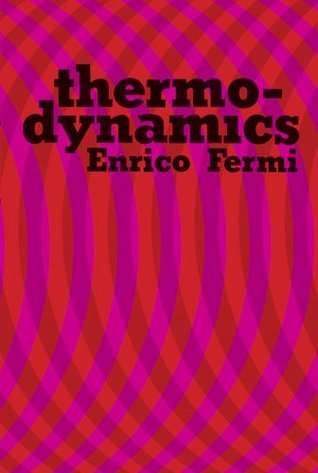
\includegraphics[width=0.35\textwidth]{figures/fermi.jpg}
\caption{Less than 10 bucks on Amazon.  Also, I have a copy.  (May assign problems for advanced students).}
\end{figure}
\end{frame}

\section{Estimation/Approximation}

\begin{frame}{Estimation/Approximation}
In science and engineering, \alert{estimation} is to obtain a quantity in the absence of precision, informed by rational constraints.
\begin{enumerate}
\item Define relevant \alert{scales}: mg, g, kg
\item Obtain \alert{complex quantities} from simple ones
\begin{itemize}
\item Obtain \textit{areas} and \textit{volumes} from \textit{lengths}
\item Obtain \textit{rates} from \textit{numerators} and \textit{denominators}
\end{itemize}
\item Constrain the unknown with \alert{upper} and \alert{lower} limits
\item Scaling problems: how does a complex quantity depend on other quantities?
\end{enumerate}
\end{frame}

\begin{frame}{Estimation/Approximation}
\small
\begin{columns}[T]
\begin{column}{0.5\textwidth}
\textbf{Choose a reasonable scale}: Estimate the mass of termites in a termite colony.  Assume that the colony is a species known to have $10^6$ individuals (roughly) per colony.
\begin{itemize}
\item A: 0.01 kg
\item B: 0.1 kg
\item C: 1 kg
\item D: 10 kg
\end{itemize}
\end{column}
\begin{column}{0.5\textwidth}
\textbf{Volume/density from other quantities}: An adult humpback whale is about 15 meters long.  What is the mass of a baby humpback whale? (1 tonne = 1000 kg).
\vspace{0.55cm}
\begin{itemize}
\item A: 100 tonnes
\item B: 50 tonnes
\item C: 10 tonnes
\item D: 2 tonnes
\end{itemize}
\end{column}
\end{columns}
\end{frame}

\begin{frame}{Estimation/Approximation}
\small
\begin{columns}[T]
\begin{column}{0.5\textwidth}
\textbf{Upper and lower bound}: The density of water is 1000 kg/m$^3$.  What is the density of ice, approximately?  (Don't think too hard!)
\begin{itemize}
\item A: 550 kg/m$^3$
\item B: 920 kg/m$^3$
\item C: 1050 kg/m$^3$
\item D: 1200 kg/m$^3$
\end{itemize}
\end{column}
\begin{column}{0.5\textwidth}
\textbf{Volumes from other quantities}: A jar at the coffee shop is filled with coffee beans, and a we can win a prize for guessing the number of beans.  If the radius of the jar is about 4 cm, and the height is about 10 cm, how many beans are in the jar?
\vspace{0.55cm}
\begin{itemize}
\item A: 200
\item B: 2,000
\item C: 10,000
\item D: Um, like, a million...
\end{itemize}
\end{column}
\end{columns}
\end{frame}

\begin{frame}{Estimation/Approximation}
\small
\begin{columns}[T]
\begin{column}{0.5\textwidth}
\textbf{Rates from other quantities}: A student travels from uptown Whittier to SLC in roughly 10 minutes.  What is her average speed?
\begin{itemize}
\item A: 0.1 m/s
\item B: 1 m/s
\item C: 5 m/s
\item D: 10 m/s
\end{itemize}
\end{column}
\begin{column}{0.5\textwidth}
\textbf{Scale}: The distance between the Earth and the sun is 1 AU.  What is the distance between the Sun and Venus?
\vspace{0.55cm}
\begin{itemize}
\item A: 10 million km
\item B: 100 million km
\item C: 0.2 AU
\item D: 0.7 AU
\end{itemize}
\end{column}
\end{columns}
\end{frame}

\begin{frame}{Estimation/Approximation}
\small
\begin{columns}[T]
\begin{column}{0.5\textwidth}
\textbf{Scaling problem}: A type of rice grain, when cooked, doubles in length.  By what factor does the volume of the grain increase?
\begin{itemize}
\item A: A factor of 2
\item B: A factor of 4
\item C: A factor of 8
\item D: A factor of 10
\end{itemize}
\end{column}
\begin{column}{0.5\textwidth}
\textbf{Scaling problem}: If the \textit{temperature} of a gas remains constant, the \textit{pressure} is inversely proportional to the volume of the gas.  If the volume of a cylinder is decreased by a factor of three, by what factor does the pressure change?
\vspace{0.55cm}
\begin{itemize}
\item A: 3
\item B: 1/3
\item C: 1
\item D: 9
\end{itemize}
\end{column}
\end{columns}
\end{frame}

\begin{frame}{Estimation/Approximation}
\small
\begin{columns}[T]
\begin{column}{0.5\textwidth}
\textbf{Unit analysis}: Which of the following are top speeds of a runner at the end of a sprint?
\begin{itemize}
\item A: 10 m/s$^2$
\item B: 30 kg m/s
\item C: 7 m/s
\item D: 20 miles per hour
\end{itemize}
\end{column}
\begin{column}{0.5\textwidth}
\textbf{Unit analysis}: Which of the following is the gravitational acceleration near the Earth's surface?
\vspace{0.55cm}
\begin{itemize}
\item A: 9.8 m/s
\item B: -9.8 m/s
\item C: -9.8 m/s/s
\item D: 9.8 m/s/s
\end{itemize}
\end{column}
\end{columns}
\end{frame}

\begin{frame}{Coordinates and Vectors - Review this separately}
\small
\begin{columns}[T]
\begin{column}{0.5\textwidth}
$\vec{p} = 4\hat{i}+2\hat{j}$.  $\vec{q} = -4\hat{i}+2\hat{j}$.  \\
Compute $\vec{p} + \vec{q}$.
\vspace{0.2cm}
\begin{itemize}
\item A: $4\hat{i}+4\hat{j}$
\item B: $0\hat{i}+4\hat{j}$
\item C: $4\hat{i}+0\hat{j}$
\item D: 0
\end{itemize}
\end{column}
\begin{column}{0.5\textwidth}
$\vec{p} = -1\hat{i}+6\hat{j}$.  $\vec{q} = 3\hat{i}+0.5\hat{j}$.  \\
Compute $\vec{p} \cdot \vec{q}$.
\vspace{0.2cm}
\begin{itemize}
\item A: -1
\item B: 1
\item C: 0
\item D: 3
\end{itemize}
\end{column}
\end{columns}
\end{frame}

\section{Kinematics and Newton's Laws}

\begin{frame}{Kinematics and Newton's Laws}
\small
\textit{Kinematics} - A \alert{description} of the motion of particles and systems \\
\textit{Dynamics} - An \alert{explanation} of the motion of particles and systems \\
\vspace{0.25cm}
What causes an object to move?  \textbf{Forces}.  Forces exist as a result of the \alert{\textbf{interactions}} of objects or systems.\\
\vspace{0.25cm}
\rule{10cm}{0.4pt} \\
\vspace{0.25cm}
\textit{Evolution} - A \alert{description} of the change of biological species \\
\textit{Natural Selection} - An \alert{explanation} of change in biological species \\
\vspace{0.25cm}
What causes species to evolve?  \textbf{Natural selection}.  Natural selection exists because of \alert{election pressures}, \alert{numerous offspring}, and \alert{variation} among offspring.
\end{frame}

\begin{frame}{Kinematics and Newton's Laws}
\textbf{Newton's First Law}: A man slides a palette crate across a concrete floor of his shop.  He exerts a force of 60.0 N, and the box has a constant velocity of 0.5 m/s.  What force cancels his pushing force, and what is the value in Newtons?
\begin{itemize}
\item A: wind, 60.0 N
\item B: friction: 60.0 N
\item C: friction: -60.0 N
\item D: weight: -60.0 N
\end{itemize}
\end{frame}

\begin{frame}{Kinematics and Newton's Laws}
\textbf{Newton's Second Law}: The crate has a mass of 50 kg, and encounters an area where there is no longer friction.  If the pushing force is still 60 N, what is the acceleration?
\begin{itemize}
\item A: 1.0 m/s/s
\item B: 0.8 m/s
\item C: 1.2 m/s
\item D: 1.2 m/s/s
\end{itemize}
\end{frame}

\begin{frame}{Kinematics and Newton's Laws}
\textbf{Kinematics}: If the acceleration is 1.2 m/s/s, and the crate begins with a velocity of 1 m/s, what is the velocity after 5 seconds?
\begin{itemize}
\item A: 4 m/s
\item B: 5 m/s
\item C: 6 m/s
\item D: 7 m/s
\end{itemize}
\end{frame}

\begin{frame}{Kinematics and Newton's Laws}
\textbf{Newton's Third Law}: Suppose the frictionless area continues indefinitely, and the velocity reaches 7 m/s.  What will be the velocity if the pushing force decreases to 0 N, when the crate has traveled 10 m?
\begin{itemize}
\item A: 7 m/s
\item B: 8 m/s
\item C: 9 m/s
\item D: 10 m/s
\end{itemize}
\end{frame}

\section{Work-Energy Theorem and Conservation of Energy}

\begin{frame}{Definitions of Work}
\begin{tcolorbox}[colback=white,colframe=red!40!blue,title=Physical Definition of Work]
\alert{Let $\vec{F}$ be a force exerted on a system, which is displaced by a displacement $\vec{x}$.  The \textbf{work} done on the system is} \\
\alert{$W = \vec{F} \cdot \vec{x}$} \\
\end{tcolorbox}
The units of work are N m = kg m/s$^2$, or \textit{Joules}. \\
\end{frame}

\begin{frame}{Definitions of Work}
Let $\theta$ be the angle between the force and the displacement.  Then this equation
\begin{equation}
W = \vec{F} \cdot \vec{x}
\end{equation}
becomes
\begin{equation}
W = Fx\cos\theta
\end{equation}
\end{frame}

\begin{frame}{Definitions of Work}
What about Newton's 3rd Law?  If one system $A$ exerts a force $F_{\rm AB}$ on a system $B$, then Newton's 3rd law states that system $B$ exerts a force $-F_{\rm AB}$ on system A. \\
\vspace{0.5cm}
If \alert{the work done by $A$ on $B$} is $W = (F_{\rm AB})x\cos\theta$, then \alert{the work done by $B$ on $A$} is $W = -(F_{\rm AB})x\cos\theta$.
\end{frame}

\begin{frame}{Definitions of Work}
What if the force varies over the trajectory of the system?  We simply have to add up each contribution along the trajectory:
\begin{equation}
W = \int_{AB} \vec{F} \cdot d\vec{r}
\end{equation}
\end{frame}

\begin{frame}{Work and Reversible Processes: the example of friction}
\small
In the first semester we encountered \textit{irreversable} processes: energy lost to \textit{friction}, and energy lost to \textit{drag}. \alert{The irreversable process is a deeper notion in thermal physics}, because it leads to the Second Law of Thermodynamics. \\ \vspace{0.5cm}
\textbf{Group board exercise}: Suppose a system moves at constant speed along a rough surface.  Draw two closed, two-dimensional paths, each describing the trajectory of the system.  A closed path means the system has a final displacement of zero.  Recall that the frictional force is not conservative.  Which path requires more work?  \textbf{Key question}: If the speed is constant the entire time, and one path requires more work than the other, what happens to the excess energy (\textit{they have the same final kinetic energy})?
\end{frame}

\begin{frame}{Kinetic Energy and the Work-Energy Theorem}
\small
The formal proof involves combining \textbf{Newton's Second Law}, and the \textbf{Definition of Work}.  Let the \textit{kinetic energy} of a particle be defined by the mass and velocity of the particle, such that $KE = \frac{1}{2}mv^2$.  Consider that
\begin{align}
W =& \int_{\rm AB} \vec{F} \cdot d\vec{x} \\
W =& \int_{\rm AB} (m\vec{a}) \cdot d\vec{x} \\
W =& m\int_{\rm AB} \left( \frac{d\vec{v}}{dt} \right) \cdot d\vec{x} \\
W =& m\int_{\rm AB} \vec{v} \cdot d\vec{v} \\
W =& \frac{1}{2}m v_{\rm B}^2 - \frac{1}{2}m v_{\rm A}^2 = \Delta KE \\
W =& \Delta KE
\end{align}
\end{frame}

\begin{frame}{Kinetic Energy and the Work-Energy Theorem}
\textbf{Group board exercise}: A firework of mass 1 kg is launched straight upwards.  The gunpowder releases 500 J of energy.  What is the velocity of the shell as it leaves the launcher?  How high does it fly straight upwards?
\end{frame}

\begin{frame}{Kinetic Energy and the Work-Energy Theorem}
\textbf{Group board exercise}: A slingshot is like a spring with a spring constant of 2000 N/m.  If a projectile is placed in the slingshot pouch, how much work is required to draw it back 10 cm? \\ \vspace{0.5cm}
\small
\textit{Actually, we learned last semester from our group projects that rubber doesn't always provide a \textbf{linear} restoring force}.
\end{frame}

\begin{frame}{Kinetic Energy and the Work-Energy Theorem}
\textbf{Group board exercise}: If the pouch is released, what is the final velocity of the projectile if all of the work is converted into kinetic energy?
\end{frame}

\begin{frame}{Definition of momentum}
Momentum is defined as follows: \\ \vspace{1cm}
\begin{tcolorbox}[colback=white,colframe=red!40!blue,title=Definition of Momentum]
\alert{A particle of mass $m$ and velocity $\vec{v}$ has the vector \textit{momentum}:} \\ \\
\alert{$\vec{p} = m\vec{v}$}
\end{tcolorbox}
\end{frame}

\begin{frame}{Definition of momentum}
There is a corollary: \\ \vspace{1cm}
\begin{tcolorbox}[colback=white,colframe=red!40!blue,title=Newton's Second Law with momentum]
\alert{If a particle has acceleration $\vec{a} = \frac{d\vec{v}}{dt}$, then} \\ \\
\alert{$\vec{F}_{\rm Net} = \frac{d\vec{p}}{dt}$}
\end{tcolorbox}
\end{frame}

\begin{frame}{Definition of momentum}
An object that has a small mass and an object that has a large mass have the same momentum. Which mass has the largest kinetic energy?
\begin{itemize}
\item A: The one with the small mass
\item B: The one with the large mass
\item C: If the momentum is the same the kinetic energy is the same
\item D: Cannot determine the answer
\end{itemize}
\end{frame}

\begin{frame}{Definition of momentum}
An object that has a small mass and an object that has a large mass have the same kinetic energy. Which mass has the largest momentum?
\begin{itemize}
\item A: The one with the small mass
\item B: The one with the large mass
\item C: If the momentum is the same the kinetic energy is the same
\item D: Cannot determine the answer
\end{itemize}
\end{frame}

\begin{frame}{Classifying collisions, and Energy Conservation}
Last semester we went into detail \alert{classifying collisions}.  For our purposes this semester, we just need to remember that collisions come in two basic forms:
\begin{itemize}
\item \textit{Elastic type}: \textbf{Both} kinetic energy and momentum are conserved.
\item \textit{Inelastic type}: Momentum is conserved.
\end{itemize}
\end{frame}

\begin{frame}{Classifying collisions, and Energy Conservation}
A puff of dust is composed of $10^6$ dust particles, each with mass of $1 \mu$g (microgram), or $10^{-6}$ grams.  The average velocity of each particle is 1 m/s.  What is the total kinetic energy, adding up the contributions from all the particles?
\begin{itemize}
\item A: $\frac{1}{2}$ mJ, or a millijoule (0.001 Joules)
\item B: $\frac{1}{2}$ $\mu$J, or a microjoule ($10^{-6}$ Joules)
\item C: 1 millijoule
\item D: 1 Joule
\end{itemize}
\end{frame}

\begin{frame}{Classifying collisions, and Energy Conservation}
What is the mass of the puff of dust, if it has $10^6$ particles each with a mass of 1 microgram?  
\begin{itemize}
\item A: 1 kilogram
\item B: 1 milligram
\item C: 1 gram
\item D: 1 $\mu$g
\end{itemize}
\end{frame}

\begin{frame}{Classifying collisions, and Energy Conservation}
Which condition will cause this number to change?
\begin{itemize}
\item A: The temperature of the puff is increased.
\item B: All of the collisions were somehow inelastic.
\item C: All of the collisions were somehow elastic.
\item D: Dust particles were removed from the puff.
\end{itemize}
\end{frame}

\begin{frame}{Classifying collisions, and Energy Conservation}
Which condition will cause the \textit{temperature} of the dust cloud to change?  (Think conceptually, from your intuition).
\begin{itemize}
\item A: The average speed of the particles increases.
\item B: The collisions are all inelastic; kinetic energy of the particles decreases on average.
\item C: The collisions are all elastic; the kinetic energy of the particles stays constant.
\item D: Dust particles were removed from the puff.
\end{itemize}
\end{frame}

\begin{frame}{Classifying collisions, and Energy Conservation}
Which condition will cause the \textit{temperature} of the dust cloud to change?  (Think conceptually, from your intuition).
\begin{itemize}
\item A: The average speed of the particles increases.
\item B: The collisions are all inelastic; kinetic energy of the particles decreases on average.
\item C: The collisions are all elastic; the kinetic energy of the particles stays constant.
\item D: Dust particles were removed from the puff.
\end{itemize}
\end{frame}

\begin{frame}{Thinking about temperature, heat, and thermal physics}
So which parts of Newtonian mechanics are we going to need to understand thermal physics? (Heat, temperature, energy transfer).
\begin{itemize}
\item Newton's laws, momentum and kinetics $\rightarrow$ motions of molecules in gases $\rightarrow$ temperature and heat
\item Work and energy $\rightarrow$ work done by thermal systems $\rightarrow$ energy conservation with heat
\item Irreversable processes $\rightarrow$ energy dissapation $\rightarrow$ entropy
\end{itemize}
\end{frame}

\section{Conclusion}

\begin{frame}{Unit 0 Summary}
\textit{Physics} - $\phi\upsilon\sigma\iota\kappa\acute{\eta}$ - "phusik\'e": \textit{knowledge of nature} \\
from $\phi\acute{\upsilon}\sigma\iota\varsigma$ - "ph\'usis": \textit{nature}
\textbf{Reading: Chapters 1 and 2 (for Unit 1)}
\begin{enumerate}
\item Estimation/Approximation
\begin{itemize}
\item \alert{Estimating} the correct order of magnitude
\item \alert{Building} complex quantities
\item \alert{Unit analysis}
\end{itemize}
\item Review of concepts from Newtonian mechanics
\begin{itemize}
\item Kinematics and \alert{Newton's Laws}
\item Work-energy theorem, energy conservation
\item Momentum, conservation of momentum
\end{itemize}
\end{enumerate}
\end{frame}

\section{Answers}

\begin{frame}{Answers}
\begin{columns}[T]
\begin{column}{0.5\textwidth}
\begin{itemize}
\item 1 kg
\item 2 tonnes
\item 2,000
\item 1 m/s
\item 100 million km or 0.7 AU
\item A factor of 8
\item 3
\item C and D
\item -9.8 m/s/s
\item $0\hat{i}+4\hat{j}$
\item 0
\end{itemize}
\end{column}
\begin{column}{0.5\textwidth}
\begin{itemize}
\item friction: -60.0 N
\item 1.2 m/s/s
\item 7 m/s
\item 7 m/s
\item The one with the small mass
\item The one with the large mass
\item $\frac{1}{2}$ mJ, or a millijoule (0.001 Joules)
\item 1 gram
\item Dust particles were removed from the puff.
\end{itemize}
\end{column}
\end{columns}
\end{frame}

\begin{frame}{Answers, continued}
\begin{columns}[T]
\begin{column}{0.5\textwidth}
\begin{itemize}
\item A and B
\end{itemize}
\end{column}
\begin{column}{0.5\textwidth}
\begin{itemize}
\item ...
\end{itemize}
\end{column}
\end{columns}
\end{frame}

\end{document}
